% -*- root: ../../main.tex -*-
\section{Design}

Come precedentemente specificato, si è deciso di procedere allo sviiluppo del sistema utilizzando il paradigma ad attori. Durante la fase di progettazione sono state designate come attori le seguenti entità:

\begin{itemize}
	\item{\textbf{Client Actor:}} è l'attore che incapsula il comportamento del client.
	\item{\textbf{Server Actor:}} è l'attore che rappresenta il server e, in quanto tale, presenta tre diversi behaviour:
		\begin{itemize}
		 	\item{\emph{Leader}}
		 	\item{\emph{Follower}} 
		 	\item{\emph{Candidate}} 
		 \end{itemize} 
	\item{\textbf{State Machine:}} è un attore figlio del Server Actor e incapsula la gestione delle richieste da eseguire e la restituzione del risultato.
\end{itemize}



\subsection{Struttura}
Il programma è composto da due sottosistemi indipendenti.

\begin{itemize}
	\item Il sottosistema \textbf{Client} è strutturato in questo modo: 
		\begin{itemize}
			\item{\textbf{Attore Client:}} che si occupa dell'interazione con i server.
			\item{\textbf{Modulo View:}} per la gestione dell'interfaccia grafica.  
		\end{itemize}
	L'interfaccia grafica, essendo un modulo univoco, è stata wrappata, per necessità, all'interno del Client. Questo, in combinazione con il \textit{pattern observer} ha permesso di \textbf{disaccoppiare} le due componenti.




	\item Il sottosistema \textbf{Server} è invece organizzato come segue:
		\begin{itemize}
			\item{\textbf{Command log:}} mantiene in memoria il log e fornisce operazioni per agire su di esso.
			\item{\textbf{BankStateMachine:}} attore che modella la macchina a stati, la quale si occupa di gestire l'esecuzione dei comandi ad essa inoltrati e la notifica dei risultati.
			\item{\textbf{Modulo di consenso:}} è la parte principale in cui si sviluppa l'algoritmo e gestisce il comportamento del server a seconda del ruolo che ricopre in un dato momento.
		\end{itemize}

\end{itemize}

\begin{figure}[H]
  \centering
  \includegraphics[width=0.99\columnwidth]{classDiagrams/serverClassCaseDiagram}
  \caption[classDiagramCaption]{Raffigurazione del diagramma delle classi lato server}
  
  \label{fig:figure27}
\end{figure}

\begin{figure}[H]
  \centering
  \includegraphics[width=0.70\columnwidth]{classDiagrams/clientClassCaseDiagram}
  \caption[classDiagramCaption]{Raffigurazione del diagramma delle classi lato client}
  
  \label{fig:figure29}
\end{figure}

Qui di seguito viene mostrato un diagramma dei componenti raffigurante i due nodi principali del cluster. Come vediamo, i nodi server sono rappresentati con una nuvola; questo sta a significare che ci troviamo in un ambiente distribuito.
\begin{figure}[H]
  \centering
  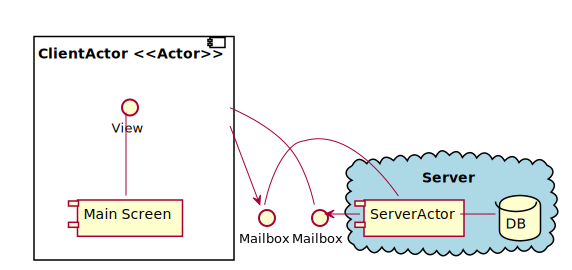
\includegraphics[width=0.99\columnwidth]{componentDiagrams/componentDiagram}
  \caption[componentDiagramCaption]{Diagramma dei componenti.}  
  \label{fig:figure30}
\end{figure}

\subsection{Comportamento}
Tra gli attori identificati nel sistema, solo uno assume, a seconda dei casi, più di un comportamento: il \textbf{Server Actor.}

Tali behaviour sono gestiti nella seguente maniera:
\begin{itemize}
	\item quando un server è \textbf{leader}, svolge le seguenti mansioni:
	\begin{itemize}
		\item \emph{\textbf{accogliere} le richieste del client, che arriveranno tramite un messaggio opportuno.}
		\item \emph{\textbf{appenderle} al proprio log, al fine di accodarle per una futura esecuzione.}
		\item \emph{\textbf{propagare} le proprie entry verso gli altri server, allo scopo di replicare il proprio log su tutti i server.} 
		\item \emph{\textbf{committare} le entry quando diventa \textbf{safe} farlo.}  
		\item \emph{\textbf{recedere} dal proprio ruolo di comando nel momento in cui si trova dinanzi a un poteziale nuovo leader, più qualificato.}
	\end{itemize}
	\item un server \textbf{follower} porta a termine i seguenti compiti:
	\begin{itemize}
		\item \emph{\textbf{appendere} le entry del leader al proprio log, quando quest'ultimo ordina di farlo.}
		\item \emph{\textbf{modificare} il proprio log, eliminando le entry non compatibili con quelle del leader, al fine di convergere al suo stesso stato.}
		\item \emph{\textbf{committare} le entry quando il leader indica di farlo.}
		\item \emph{\textbf{ridirigere} il client, comunicando l'identità del leader, in caso si riceva una richiesta.}
		\item \emph{\textbf{votare} per i candidati che richiedono un voto, esprimendo un giudizio positivo o negativo, a seconda del soddisfacimento delle condizioni necessarie.}		\item \emph{\textbf{candidarsi} come potenziale leader nel momento in cui si perdono i contatti con quello corrente e si assume, di conseguenza, che sia attualmente irraggiungibile.}
	\end{itemize}

	\item un server in modalità \textbf{candidato} esegue le seguenti operazioni:
	\begin{itemize}
		\item \emph{\textbf{inviare} richieste di voto agli altri server.}
		\item \emph{\textbf{contare} le risposte positive e cambiare il proprio stato in \textbf{leader} in caso di maggioranza dei voti.}
		\item \emph{\textbf{recedere} a \textbf{follower} nel caso in cui le elezioni siano vinte da qualcun altro.}
		\item \emph{\textbf{ricandidarsi} una seconda volta nel caso in cui, allo scadere di un timer, non si sia raggiunta la maggioranza dei voti nè si sia venuti a conoscenza dell'avvenuta elezione di un nuovo leader.}			  		
	\end{itemize}
\end{itemize}


\subsection{Interazione}
Qui di seguito verranno elencati i principali messaggi che vengono scambiati tra i vari attori:

	\subsubsection{RAFT Protocol}
		\begin{itemize}
			\item{\texttt{AppendEntries(leaderTerm, previousEntry,entry,\\
			 leaderLastCommit) }}
			\item{\texttt{AppendEntriesResult(success, matchIndex, followerTerm) }}
			\item{\texttt{RequestVote(candidateTerm, candidateId, lastLogTerm,\\
			 lastLogIndex)}}
			\item{\texttt{RequestVoteResult(voteGranted, followerTerm)}}
			\item{\texttt{ClientRequest(requestId, command)}}
			\item{\texttt{RequestResult(requestiId, success, result)}}
			\item{\texttt{Redirect(requestId, leaderRef)}}
		\end{itemize}

	\subsubsection{Control Protocol}
		\begin{itemize}
			\item{\texttt{GuiSendMsg(serverId, commandType, iban, amount)}}
			\item{\texttt{GuiStopServer(serverId)}}
			\item{\texttt{GuiResumeServer(serverId)}}
			\item{\texttt{GuiTimeoutServer(serverId)}}
			\item{\texttt{GuiMsgLossServer(serverId, loss)}}
		\end{itemize}